\documentclass[12pt, a4paper]{article}

%%%% Shape

%\usepackage{geometry}
 %\geometry{
 %a4paper,
 %total={170mm,257mm},
 %left=20mm,
 %top=20mm,
 %}

%%%% Encodings
\usepackage[utf8]{inputenc} % encoding
\usepackage[english]{babel} % use special characters and also translates some elements within the document.

%%%% Misc

\usepackage{hyperref}       % Hyperlinks \url{url} or \href{url}{name}
\usepackage{parskip}        % \par starts on left (not idented)
\usepackage{tocbibind}      % Adds the bibliography to the table of contents (automatically)

% \usepackage[document]{ragged2e}  % Left-aligned (whole document)
% \begin{...} ... \end{...}   flushleft, flushright, center

%%%% Abstract

\usepackage{abstract}       % Abstract

% http://www.ctex.org/documents/packages/special/abstract.pdf
\renewcommand{\absnamepos}{flushleft} % \begin{abstract} \noindent ... \end{abstract}
\setlength{\absleftindent}{0pt}
\setlength{\absrightindent}{0pt}

%%%% Graphics

\usepackage{graphicx}
\graphicspath{ {./figs/} } % directory to look up for graphics

% \begin{figure}[h]
%   \centering
%   \includegraphics[scale=0.5]{cat}  % [width=\textwidth, height=4cm],
%   \caption{Example of a cat}
%   \label{fig:cat}
% \end{figure}

%%%% Math

\usepackage{amsmath}        % Math
\usepackage{amssymb}        % New symbols http://milde.users.sourceforge.net/LUCR/Math/mathpackages/amssymb-symbols.pdf
\usepackage{bm}             % $\bm{D + C}$

\usepackage{amsthm} % Math, \newtheorem, \proof, etc
% \begin{theorem}\label{t:label}  ...  \end{theorem}
% \begin{proof} ... \end{proof}
\theoremstyle{plain} % default
\newtheorem{theorem}{Theorem}[section]
\newtheorem{corollary}{Corollary}[theorem]  % Numering depends on the current section (instead of global)
\newtheorem{lemma}[theorem]{Lemma} % Shares numeration with theorem.
\theoremstyle{definition}
\newtheorem{definition}{Definition}[section]
\theoremstyle{remark}
\newtheorem*{remark}{Remark}

% Defines a new environment to write your or claim - proof
\newenvironment{claim}[1]{\par\noindent\underline{Claim:}\space#1}{}
\newenvironment{claimproof}[1]{\par\noindent\underline{Proof:}\space#1}{\hfill $\blacksquare$}

%%%% Code/Pseudo-code

\usepackage{minted} % Code listing
% \mint{html}|<h2>Something <b>here</b></h2>|
% \inputminted{octave}{BitXorMatrix.m}

%\begin{listing}[H]
  %\begin{minted}[xleftmargin=20pt,linenos,bgcolor=codegray]{haskell}
  %\end{minted}
  %\caption{Example of a listing.}
  %\label{lst:example} % You can reference it by \ref{lst:example}
%\end{listing}

\newcommand{\code}[1]{\texttt{#1}} % Define \code{foo.hs} environment

\usepackage[vlined,ruled]{algorithm2e} % pseudo-code http://tug.ctan.org/macros/latex/contrib/algorithm2e/doc/algorithm2e.pdf

%%%% Colors

\usepackage{xcolor}         % Colours \definecolor, \color{codegray}
\definecolor{codegray}{rgb}{0.9, 0.9, 0.9}
% \color{codegray} ... ...
% \textcolor{red}{easily}

%%%% Math

%\makeglossaries % before entries

%\newglossaryentry{latex}{
    %name=latex,
    %description={Is a mark up language specially suited
    %for scientific documents}
%}

% Referene to a glossary \gls{latex}
% Print glossaries \printglossaries

\usepackage[acronym]{glossaries} %

% \acrshort{name}
% \acrfull{name}
% \newacronym{foo}{arcshort}{acrfull}

\usepackage{enumitem} % \begin{enumerate}[label=(\alph*)]



\usepackage{fancyhdr}
\pagestyle{fancy}
\fancyhf{}
\rhead{TOML}
\lhead{}
\rfoot{Page \thepage}

\title{%
  \vspace{-10ex}
  TOML: Programming Exercises
}
\author{%
  Arnau Abella \\
  \large{Universitat Polit\`ecnica de Catalunya}
}
\date{\today}

\begin{document}
\maketitle

%%%%%%%%%%%%%%%%%%%%%%%%%%%%%%

\section*{Exercise 1}%
\label{sec:exercise_1}

\begin{enumerate}[label={(\alph*)}, ref=\arabic*, leftmargin=0cm]
  \item We can check convexity by checking the second-order conditions.

    \begin{align*}
      &f(x_1,x_2) = e^x_1(4x_1^2+2x_2^2+4x_1x_2+2x_2+1) \\
      &(\frac{\partial f}{\partial x_1}, \frac{\partial f}{\partial x_2}) =
        (e^{x_1}(4x_1^2+4x_1(x_2+2)2x_2^2 + 6x_2 + 1, \ e^x_1(4x_1 + 4x_2+2))\\
      & H_f = \begin{bmatrix}\frac{\partial^2 f}{\partial x_1^2} & \frac{\partial^2 f}{\partial x_1 \partial x_2} \\ \frac{\partial^2 f}{\partial x_2 \partial x_1} & \frac{\partial^2 f}{\partial x_2^2}\end{bmatrix} = \begin{bmatrix}e^x_1(4x_1^2 + 4x_1(x_2  + 2) + 2x_2^2 + 10x_2 + 9) & e^x_1(4x_1 + 4x_2 + 6) \\ 2e^x_1(2x_1 + 2x_2+3) & 4e^x_1 \end{bmatrix}
    \end{align*}

    The Hessian matrix it is not positive nor negative semidefinite. Therefore, $f(x_1,x_2)$ is not convex nor concave.

\begin{figure}[H]
  \centering
  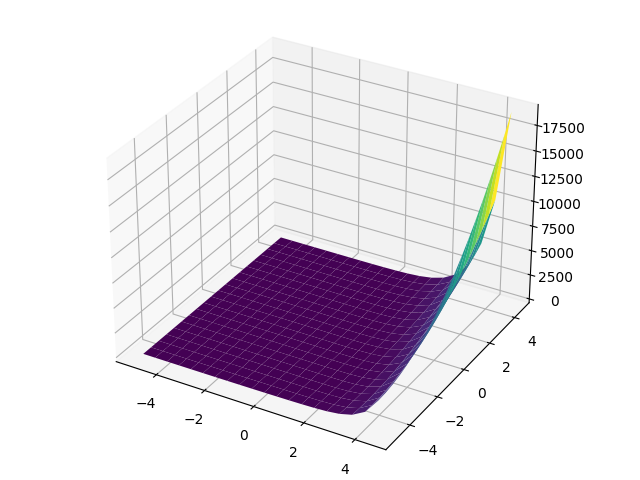
\includegraphics[width=0.7\textwidth]{exercise1_plot.png}
  \label{fig:exercise1}
  \caption{3D plot of $f(x_1,x_2) = e^x_1(4x_1^2+2x_2^2+4x_1x_2+2x_2+1)$}
\end{figure}

\newpage

  \item Depending on the starting point we get different optimal points since the objective function is not convex (see plot ~\ref{fig:exercise1}).

\begin{table}[H]
\centering
\begin{tabular}{c|c|c|c}
$x_0$                           & $x*$                                & $p*$                              & Iter.                  \\ \hline
(0, 0)                          & (-24.9, 45.4)                       & $3.29e^{-8}$                      & 6                      \\
(10, 20)                        & (-0.0047, 8.95)                     & $0.0$                             & 2                      \\
(-10, 1)                        & (-28.1, 21.4)                       & $1.03e^{-9}$                      & 28                     \\
(-30, -30)                      & (-28.5, 10.46)                      & $9.5e^{-10}$                      & 34                     \\
\end{tabular}
\end{table}

  \item The method has speed up (see table \ref{table:exercise1_times})

\begin{table}[H]
\centering
\begin{tabular}{c|c|c}
$x_0$      & Execution time & Execution time (with jacobi) \\
(0, 0)     & 0.0032"        & 0.00185" \\
(10, 20)   & 0.0014"        & 0.0011" \\
(-10, 1)   & 0.0094"        & 0.0065" \\
(-30, -30) & 0.011"         & 0.0077" \\
  \label{table:exercise1_times}
\end{tabular}
\end{table}

\begin{listing}[H]
  \inputminted[breaklines=true,fontsize=\footnotesize]{python}{../exercise1_plot.py}
  \label{lst:exercise1_plot}
  \caption{Code used for ploting exercise 1.}
\end{listing}

\begin{listing}[H]
  \inputminted[breaklines=true,fontsize=\footnotesize]{python}{../exercise1.py}
  \label{lst:exercise1}
  \caption{\code{exercise1.py}}
\end{listing}

\end{enumerate}

%%%%%%%%%%%%%%%%%%%%%%%%%%%%%%

\newpage
\section*{Exercise 2}%
\label{sec:exercise_2}

\begin{enumerate}[label={(\alph*)}, ref=\arabic*, leftmargin=0cm]
  \item We can check convexity by checking the second-order conditions.

    \begin{align*}
      &f(x_1,x_2) = x_1^2+x_2^2 \\
      &(\frac{\partial f}{\partial x_1}, \frac{\partial f}{\partial x_2}) = (2x, 2y)\\
      & H_f = \begin{bmatrix}\frac{\partial^2 f}{\partial x_1^2} & \frac{\partial^2 f}{\partial x_1 \partial x_2} \\ \frac{\partial^2 f}{\partial x_2 \partial x_1} & \frac{\partial^2 f}{\partial x_2^2}\end{bmatrix} = \begin{bmatrix}2 & 0\\0 & 2\end{bmatrix}
    \end{align*}

    Alternatively, you can check if $P \geq 0$ in the quadratic form $\frac{1}{2}x^TPx+q^Tx+r$.

    \begin{align*}
      &f(x_1, x_2) = x_1^2+x_2^2 = \begin{bmatrix}x_1 & x_2\end{bmatrix}\begin{bmatrix}1 & 0\\0 & 1\end{bmatrix}\begin{bmatrix}x_1\\x_2\end{bmatrix}
    \end{align*}

    where $P = \begin{bmatrix}1 & 0\\0 & 1\end{bmatrix} \geq 0$

    The Hessian matrix is positive and all inequalities are convex. Therefore, $f(x_1,x_2)$ is positive semi-definite.

\begin{figure}[H]
  \centering
  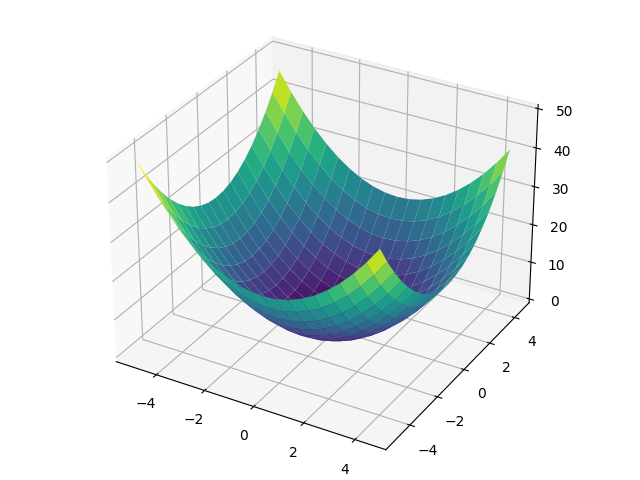
\includegraphics[width=0.7\textwidth]{exercise2_plot.png}
  \label{fig:exercise2}
  \caption{3D plot of $f(x_1,x_2) = x_1^2+x_2^2$}
\end{figure}

\newpage

  \item The result for the feasible initial point is $x* = (1.0, 1.0)$ and $p* \approx 2$. For the unfeasible initial point, the algorithm exits giving the initial point. The number of steps untill convergence is $13$. The code for this exercise can be found at \code{exercise2.py} and \code{exercise2\_plot.py}.

  \item The number of steps with giving the Jacobian as an input is $14$ but the number of functions is $14$, way smaller than before ($67$). My hypothesis is that the giving initial point is near the optimal solution and so the number of steps is small. Probably, the approximation of the Jacobian is also good.

\end{enumerate}

%%%%%%%%%%%%%%%%%%%%%%%%%%%%%%

\newpage
\section*{Exercise 3}%
\label{sec:exercise_3}

We can check convexity by checking the second-order conditions of the objective function and the inequalities. We have already checked the convexity of $f(x_1,x_2) = x_1^2+x_2^2$ and its domain. Then, we only need to check the convexity of the inequalities. The second inequality is convex since it is linear and $x_1^2 + x_1x_ + x_2^2 \leq 3$ is a quadratic equation with $P \geq 0$, so it is convex.

\begin{figure}[H]
  \centering
  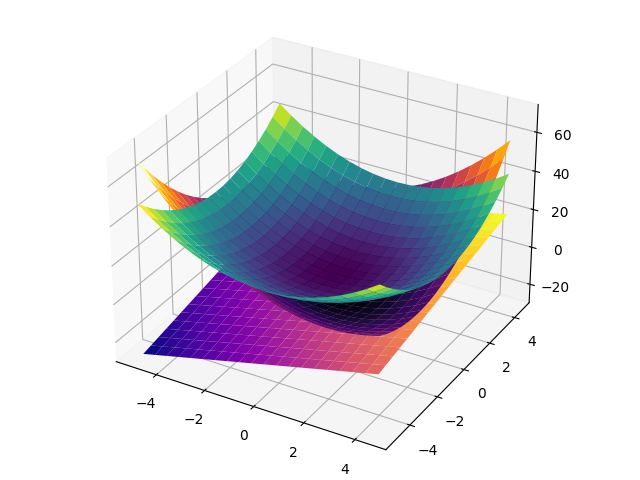
\includegraphics[width=1\textwidth]{exercise3_plot.png}
  \label{fig:exercise3}
  \caption{3D plot of the COP}
\end{figure}

The optimal point is $x* = (0.69230769, 0.46153846)$ with optimal value $p* = 0.6923076923076928$. The convergence is after 3 iterations since $x_0 = (0, 0)$.

%%%%%%%%%%%%%%%%%%%%%%%%%%%%%%

\newpage
\section*{Exercise 4}%
\label{sec:exercise_4}

\begin{listing}[H]
  \inputminted[breaklines=true,fontsize=\footnotesize]{python}{../exercise4.py}
  \label{lst:exercise4}
  \caption{\code{exercise4.py}}
\end{listing}


%%%%%%%%%%%%%%%%%%%%%%%%%%%%%%

\newpage
\section*{Exercise 5}%
\label{sec:exercise_5}

\begin{listing}[H]
  \inputminted[breaklines=true,fontsize=\footnotesize]{python}{../exercise5.py}
  \label{lst:exercise5}
  \caption{\code{exercise5.py}}
\end{listing}

%%%%%%%%%%%%%%%%%%%%%%%%%%%%%%

\newpage
\section*{Exercise 6}%
\label{sec:exercise_6}



%%%%%%%%%%%%%%%%%%%%%%%%%%%%%%

\newpage
\section*{Exercise 7}%
\label{sec:exercise_7}



%%%%%%%%%%%%%%%%%%%%%%%%%%%%%%

\newpage
\section*{Exercise 8}%
\label{sec:exercise_8}



%%%%%%%%%%%%%%%%%%%%%%%%%%%%%%

\end{document}
